\section{Network (Sergey)}

CLAS12 network is shown on Fig.~\ref{fig:network_diagram}. Its main component is Arista router serving as backbone for entire system. Set of main DAQ servers connected directly to that router by 40Gbit links. Some front-end components with high data rate connected directly to the router by 10Gbit links. Most of front-end conponents, as well as workstations are connected to the network switches using 1Gbit links, while those switches are connected to the router by 10Gbit links. Two 40Gbit uplinks connects entire system to the JLAB computer center.

Most of 1Gbit links uing copper wires while 10Gbit and 40Gbit ones using optic fibers, with the exception of short range server links where 40Gbit wires are used.

CLAS12 network shows adequate performance and high level of reliability. With projected data rates, it can be used 'as is' for the number of years.

\begin{figure}[hbt]
	\centering
	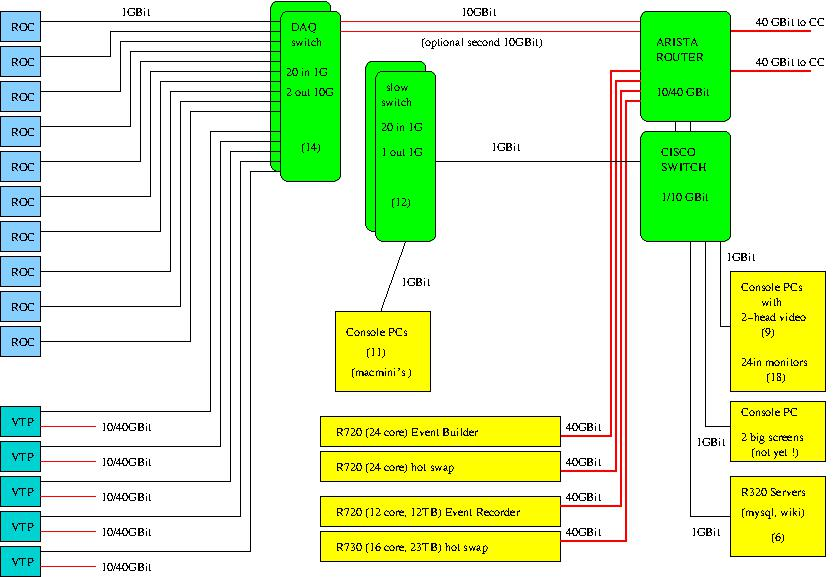
\includegraphics[width=1.0\columnwidth,keepaspectratio]{img/CLAS12_NET_1.jpg}
	\caption{CLAS12 DAQ Network Diagram}
	\label{fig:network_diagram}
\end{figure}
